\part{Transaction fundamentals}
\textit{Disclaimer: This part is not very good pedagogically. It is unclear what the context is for the terminology and methodology used. It seems to be based around JAVA infrastructure or something. The notes I have therefore are unable to give any decent intuition and are more used as a high-level explanatory thingy for when questions regarding this appears on exams.}

\section{Learning Goals}
\begin{itemize}
\item Knowledge of eight “design patterns” (Locking, Two-Phase Commit, Transaction Manager, Resource Manager, Log, Checkpoints, Log Manager, Lock Manager), how they work and which problems they solve. Ability to utilize these patterns in high-level design. 
\item Comprehension of terms: Optimistic Concurrency Control, Two-phase commit optimizations, Heuristic Transactions, Interposition.
\end{itemize}

\section{Motivation and context}
\begin{itemize}
\item We need error handling and containment for systems with multiple participants (threads, processes, distributed systems). These participants must often cooperate in the error handling.
\item Transactions (and atomic actions) are techniques/frameworks that provide the means to do this. They fall under the category of dynamic SW redundancy. 
\item Transactions contribute towards the desired error assessment and confinement design and help avoid the \textit{domino effect}
\end{itemize}

We will learn Transaction fundamentals through \textbf{eight design patterns} and some additional terms. Before we get into that note that a transaction is an indivisible, atomic action with backward error recovery. The properties of a transaction described by \textit{ACID properties}
\begin{itemize}
\item \textbf{Atomicity} -  The transaction either commits successfully or aborts completely.
\item \textbf{Consistency} - Transactions preserve a consistent state.
\item \textbf{Isolation} - Intermediate states during a transaction are not visible from the outside. Furthermore, transactions appear to be executing serially even when they are not.
\item \textbf{Durability} - The effects of a commited transition are never lost, they are stored in stable storage such as a hard drive.
\end{itemize}

With backward error recovery the flow of control of a single-threaded program is as follows:
\begin{verbatim}
allocate locks
create recovery point
do work(goto end if any problems)
label end:
if (error) {
	roll back to recovery point
    status=FAIL
} else {
    status=OK
}
release locks
return status
\end{verbatim}
It should be noted that the acceptance test that is responsible for detecting the errors in the program above.

The workings of a transaction can be further visualized by a sequence diagram. It can be a good idea to read about the eight design patterns and come back to this figure. 
\begin{figure}[H]
\centering
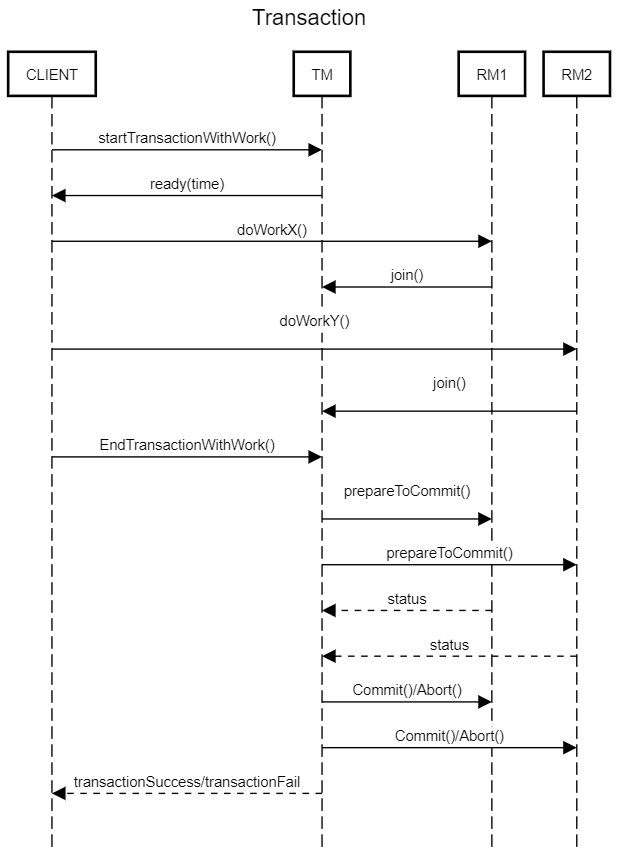
\includegraphics[width=0.6\textwidth]{figures/Fault_Tolerance/TransactionSequence.png}
\end{figure}

\section{The 8 design patterns}
\subsection{Two-phase commits}
Associated with each transaction is a coordinator/Transaction Manager, that communicates with the participants. The message flow is as follows:
\begin{verbatim}
Coordinator                                          Participant
                             QUERY TO COMMIT
                 -------------------------------->
                             VOTE YES/NO             prepare*/abort*
                 <-------------------------------
commit*/abort*               COMMIT/ROLLBACK
                 -------------------------------->
                             ACKNOWLEDGMENT          commit*/abort*
                 <--------------------------------  
end
\end{verbatim}
\subsubsection{Basic Algorithm}
Commit request (or voting) phase 
\begin{enumerate}
\item Coordinator sends \textbf{query to commit} and waits until has received reply from all participants
\item Participants execute transaction up to the point where they will be asked to commit. Each write entry to undo lo and redo log.
\item Participants vote \textbf{Yes} if their actions succeeded or \textbf{No} if they have experienced a failure making it impossible to commit.
\end{enumerate}
Commit/Completion phase
\begin{itemize}
\item \textbf{Success} - All participants voted yes. Coordinator responds with commit instruction.
\item \textbf{Failure} - At least one participant voted no. Coordinator responds with rollback instruction.
\end{itemize}

Note that: A disadvantage with two-phase commits is that the protocol is blocking. Participants will block after they have voted, awaiting a commit or rollback
message. If the coordinator fails, they will never receive either.

\subsection{Locking}
Ensures that intermediate states are not propagated. Additionally, ensures that participants can only communicate with other participants. The participant must be part of the ongoing transaction to be able to use the locked resource. 

\subsection{Lock Manager}
Can have the following functionality:
\begin{itemize}
\item Release all locks associated with transaction X when it finishes.
\item Tidy up after restart (open locks that should be open etc.)
\item Handle resources shared by several Resource Managers.
\item Include deadlock avoidance and detection algorithms.
\end{itemize}
Can also have other functions relating to locks.

\subsection{Resource Manager}
The resource managers are the \textit{transaction participants}. 
\begin{itemize}
\item Keeps track of locks and recovery points
\item Communicates with transaction manager during voting and commit phases.
\end{itemize}

\subsection{Transaction Manager}
Useful if there are multiple participants
\begin{itemize}
\item Creates the transaction, keeps track of participants
\item Plays the role of coordinator
\item Can provide a transaction deadline and abort if the deadline is missed.
\end{itemize}

\subsection{The log}
\begin{itemize}
\item Alternative to checkpoints
\item Every participant including the TM writes every planned change of state to the log and waits until the operation is confirmed safe to perform it. 
\item Processes can restore state after restart by executing the logrecords.
\item Logrecords can be executed backwards to undo actions, therefore no need for checkpoints.
\end{itemize}

\subsection{The Log manager}
Queues logrecords, optimizes disk access and sends acknowledgments receipts on received log records.

\subsection{Checkpoints}
Discussed before, alternative to log method described above. Stores a consistent state that we can start the system in.

\section{Other terms}
\subsection{Optimistic concurrency control:}
This method assumes that multiple transactions can frequently complete without interfering with each other. While running, transactions use resources without utilizing locks or other synchronization primitives. This works because before committing, each transaction verifies that no other transaction has modified the data it has read. If conflicting modifications are revealed, the transaction is rolled back and restarted. OCC can work well when we have low data contention, meaning when conflicts are rare

\subsection{Two-phase commit optimizations}
Different methods exist here
\begin{itemize}
\item Early abort using e.g. ATC
\item One-phase when only one participant
\item Read-only operations will never be aborted thus will always yield commit.
\item Last resource commit: One participant gets to wait until all the other votes are in and take these into consideration before making its vote.
\end{itemize}

\subsection{Heuristic transactions}
What if we give our vote and then loose connection? We have to make local guess and maybe to forward error recovery after.

\subsection{Interposition}
The TM's ability to play the role of a RM.
